\documentclass[10pt]{standalone}
%\usepackage[utf8]{inputenc}
\usepackage{pgfplots}
\pgfplotsset{compat=1.15}
\usepackage{mathrsfs}
\usetikzlibrary{arrows}
\pagestyle{empty}
\begin{document}

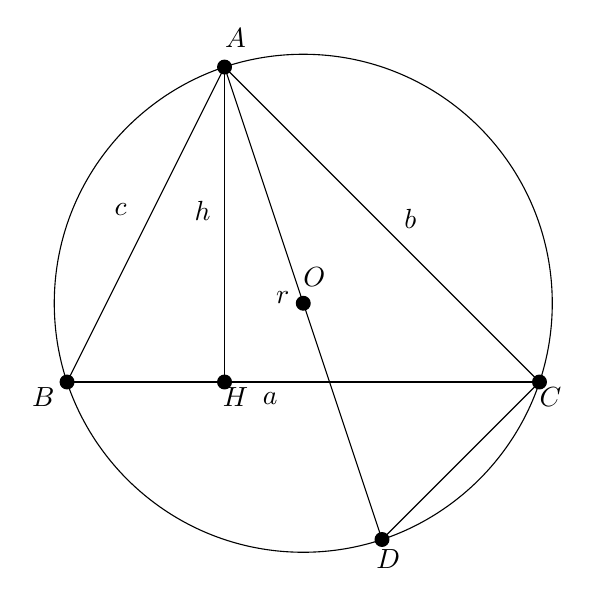
\begin{tikzpicture}[line cap=round,line join=round,>=triangle 45,x=1.0cm,y=1.0cm]
\clip(1.5,-2.5) rectangle (8.5,4.5);
\draw  (4.,4.)-- (8.,0.);
\draw  (8.,0.)-- (2.,0.);
\draw  (2.,0.)-- (4.,4.);
\draw  (5.,1.) circle (3.1622776601683795cm);
\draw  (8.,0.)-- (6.,-2.);
\draw  (4.,4.)-- (6.,-2.);
\draw  (4.,4.)-- (4.,0.);

\draw [fill=black] (4.,4.) circle (2.5pt);
\draw[color=black] (4.14,4.37) node {$A$};
\draw [fill=black] (8.,0.) circle (2.5pt);
\draw[color=black] (8.14,-0.19) node {$C$};
\draw [fill=black] (2.,0.) circle (2.5pt);
\draw[color=black] (1.7,-0.19) node {$B$};
\draw[color=black] (6.36,2.07) node {$b$};
\draw[color=black] (4.58,-0.21) node {$a$};
\draw[color=black] (2.68,2.19) node {$c$};
\draw [fill=black] (5.,1.) circle (2.5pt);
\draw[color=black] (5.14,1.33) node {$O$};
\draw [fill=black] (6.,-2.) circle (2.5pt);
\draw[color=black] (6.08,-2.25) node {$D$};
\draw[color=black] (4.74,1.07) node {$r$};
\draw [fill=black] (4.,0.) circle (2.5pt);
\draw[color=black] (4.14,-0.19) node {$H$};
\draw[color=black] (3.72,2.17) node {$h$};
\end{tikzpicture}
\end{document}